%%%%%%%%%%%%%%%%%%%%%%%%%%%%%%%%%%%%%%%%%%%%%%%%%%%%%%%%%%%%%%%%%%%%%%%%%%%%%%%%%%%%%%%%%%%%%%%%%%%
% Chapter 5 -> PHLOWER Experiments and Results
% Author: Mingbo Cheng
%%%%%%%%%%%%%%%%%%%%%%%%%%%%%%%%%%%%%%%%%%%%%%%%%%%%%%%%%%%%%%%%%%%%%%%%%%%%%%%%%%%%%%%%%%%%%%%%%%%
\chapter{PHLOWER Experiments \& Results}
\label{chapter:PHLOWER_bench}

\graphicspath{{chapter5/figs}}

\section{Experiments}
\subsection{Evaluation of trajectory inference}
\subsection{Simulated Data}
\subsection{Execution of trajectory inference}
% List how to install and run the competing methods
% how to set up dynverse environment
\subsubsection{competing methods}
	We first, install dyno(0.1.2) which includes some competing methods of wrapping. To do this, we use devtools::install\_github(``dynverse/dyno'') which includes the dynverse packages dynwrap(1.2.3),  dynmethods(1.0.5.9000), dynplot(1.1.2) and dynfeature(1.0.0). For PHLOWER and STREAM wrapping, we followed tutorial ~\url{https://dynverse.org/developers/creating-ti-method/}. For this, we clone dynclipy(0.1) code from ~\url{https://github.com/dynverse/dynclipy} and use ``pip install .'' to install the package.
\begin{description}
	\item[PHLOWER]
	We need use 
	\item[TSCAN]
	TSCAN has been wrapped in dynmethods, we just pass the ti\_tscan function to dynwrap function infer\_trajectory to infer the trajectory. source code is ~\url{https://github.com/dynverse/ti\_tscan}
	\item[STREAM]
	\item[PAGA] 
	PAGA has been wrapped in dynmethods, we just pass ti\_paga\_tree function to dynwrap function infer\_trajectory to infer the trajectory. source code is ~\url{https://github.com/dynverse/ti\_paga\_tree}
	\item[Monocle3]
	Monocle3 has been wrapped in dynmethods, we just pass the ti\_monocle3 function to dynwrap function infer\_trajectory to infer the trajectory. source code is ~\url{https://github.com/dynverse/ti\_monocle3}
	\item[Slingshot]
	Slingshot has been wrapped in dynwmethods, we just pass ti\_slingshot function to dynwrap function infer\_trajectory to infer the trajectory. source code is ~\url{https://github.com/dynverse/ti\_slingshot}
	\item[Slicer]
	xxx
	\item[slice]
	Slice has been wrapped in dynmethods in ~\url{https://github.com/dynverse/ti\_slice}. However, the simulated data need not log transformation, we adjust ti\_slice code to exclude the transformation part i.e. set ``expression <- exp(expression) - 1'' to be a new wrapper method\_slice. And pass method\_slice function to dynwrap function infer\_trajectory to infer the trajectory.
	\item[RaceID/StemID]
	RaceID/StemID has been wrapped in dynmethods in ~\url{https://github.com/dynverse/ti\_raceid\_stemid}. However, it needs positive input, we adjust ti\_raceid\_stemid code to scale the input data to 0-10 to be a new wrapper method\_raceid\_stemid. And pass method\_raceid\_stemid function to dynwrap function infer\_trajectory to infer the trajectory.
	\item[MST] 
	Minimum spanning tree(MST) is implemented in R package mclust.
	\item[ElPiGraph] 
	ElPigraph has been wrapped in dynmethods, we just pass the ti\_elpigraph function to dynwrap function infer\_trajectory to infer the trajectory. source code is ~\url{https://github.com/dynverse/ti_elpigraph}
	\item[celltree] 
	celltree has been wrapped in dynmethods in ~\url{https://github.com/dynverse/ti\_celltree\_vem}. However, the cellTree source code normalization function ``.normalise.data'' would not work with negative values. We check out cellTree(1.27.0) source code from ~\url{https://git.bioconductor.org/packages/cellTree} and adjust the ``.normalise.data'' function to use 0-1 normalization as the data output for the downstream inference process and recompile cellTree package as the input of dynmethods wrapper. We re-wrap ti\_celltree\_vem code to use the call new cellTree package to be a new wrapper method\_celltree\_vem. And pass method\_celltree\_vem function to dynwrap function infer\_trajectory to infer the trajectory.
	\item[pCreode] 
	pCreode has been wrapped in dynmethods, we just pass the ti\_pcreode function to dynwrap function infer\_trajectory to infer the trajectory. source code is ~\url{https://github.com/dynverse/ti\_pcreode}
\end{description}

\subsection{Biological Validation}

%\subsection{Single Cell Kidney Organoids}

\subsubsection{Ethical statement}

Human adult skin fibroblasts derived from a healthy volunteer, after giving informed consent, were used to generate iPSCs. This study was conducted in accordance with the Helsinki Declaration as revised in 2013. Permission for the creation and use of iPSCs in this study was obtained from the local ethical commission for human-related research of the Radboud University Medical Center, Nijmegen (approval numbers: 2015-1543 and 2006-048). 

\subsubsection{Cell culture}

Human adult skin fibroblasts derived from a healthy volunteer were reprogrammed into iPSCs using the Yamanaka factors \cite{takahashi2006induction} by the Stem Cells Technology Center at Radboud University Medical Center (SCTC, Radboud UMC, Nijmegen, The Netherlands). The iPSCs used in the current study were generated from spare materials from a healthy donor, who did consent with the use of such material and did not suffer from kidney disease. The materials have been anonymized and were collected during a time in which no signed informed consent was required.

Generation of human induced pluripotent stem cell (iPSC) derived kidney organoids iPSC were seeded using a density of 18,000 cells/cm2 on Geltrex (Thermo Fisher, Breda, the Netherlands) coated 6-well plates (Greiner Bio-one, Alphen aan de Rijn, the Netherlands). The differentiation protocol was based on our previous work \cite{jansen2022sars}. In brief, differentiation towards ureteric bud-like and metanephric mesenchyme lineage was initiated using CHIR-99021 (6 $\mu$M, R\&D systems, Abingdon, United Kingdom) in Essential 6 medium (Thermo Fisher, Breda, The Netherlands) for 3 and 5 days, respectively. Next, medium was  replaced sequentially for Essential 6 supplemented with fibroblast growth factor 9 (FGF9), 200 ng/ml, R\&D systems) and heparin (1 $\mu$g/ml, Sigma-Aldrich, Zwijndrecht, Netherlands) up to day 7. On day 7, differentiated cells were trypsinized and mixed in a ratio of one part 3 days CHIR-differentiated cells and two parts 5 days CHIR-differentiated cells to stimulate crosstalk between both lineages in order to boost segmented nephrogenesis. To generate cell pellets, 300,000 cells per 1.5 ml tube were aliquoted from the cell mix and centrifuged 3 times at 300 rcf for 3 min changing position by 180$^\circ$ per cycle. Cell pellets were plated on Costar Transwell filters (type 3450, Corning, Sigma-Aldrich), followed by a one-hour CHIR pulse (5 $\mu$M) in Essential 6 medium added to the basolateral compartment. Next, medium was replaced for Essential 6 medium supplemented with FGF9 and heparin for additional 5 days, and the entire 3D organoid culture was performed using the air-liquid interface. After 5 days of organoid culture, Essential 6 medium supplemented with human epidermal growth factor (hEGF, 10 ng/ml, Sigma-Aldrich), bone morphogenetic protein-7 (BMP7, 50 ng/ml, R\&D systems), stromal derived factor 1 beta (SDF1$\beta$, 10 ng/ml, R\&D systems), vasopressin (10 nM, Sigma-Aldrich), aldosterone (10 nM, Sigma-Aldrich) was used. Medium was replaced every other day for an additional 13 days. 

Harvesting kidney organoids for 10x genomics NEXT GEM multiome pipeline
To dissect nephrogenic differentiation trajectories in kidney organoids using the multiome pipeline, organoids were harvested at different time points during culture. The following differentiation stages were processed:  day 7 (cells harvested from the 2D cell layer, primitive streak - intermediate mesoderm stage), organoids day 7+5, day 7+12 and day 7+18. These kidney organoid stages represent nephrogenesis ranging from intermediate mesoderm (day 7+5) towards metanephric mesenchyme and ureteric bud-like lineages (day 7+12) that result into nephron-like structures embedded by a (progenitor) stromal compartment at the end of the differentiation protocol (day 7+18). Kidney organoids were harvested on the respective dates (d7+5, d7+12, and d7+18) by cutting single organoids out of the transwell filter in a sterile flow hood using a scalpel. Organoids were washed with 5 ml PBS per filter at room temperature 3 times. Afterwards, single organoids were cut from the transwell filter with the organoids still being attached to the membrane, transferred to 1.7 ml cryovials (Greiner bio-one) and subsequently snap frozen and stored at -80$^\circ$ until nuclei isolation. 

\subsubsection{Single nuclei isolation from kidney organoids}

Snap-frozen kidney organoids were thawed in PBS and crushed using a glass tube and douncer (Duran Wheaton Kimble Life Sciences, Wertheim/Main, Germany). After passing the single cell suspension through a 40 $\mu$m cell strainer (Greiner bio-one), the suspension was centrifuged at 4$^\circ C$ and 300xg for 5 min. Subsequently, the supernatant was discarded and the cell pellet was resuspended in Nuc101 cell lysis buffer (Thermo Fisher), supplemented with RNase and protease inhibitors (Recombinant RNase Inhibitor and Superase RNase Inhibitor, Thermo Fisher, and Complete Protease Inhibitor, Roche), incubated for 30 seconds and centrifuged at 4$^\circ$ and 500xg for 5 min. After discarding the supernatant, the nuclei were carefully resuspended in PBS containing 1\% (v/v) Ultra-Pure BSA (Invitrogen Ambion, Thermo Fisher) and Protector RNAse inhibitor (Sigma Aldrich). Single nuclei were counted using Trypan blue (Thermo Fisher) and prepared for 10x genomics ChromiumNextGEM Multiome pipeline v1 according to the manufacturers guidelines (~\url{https://cdn.10xgenomics.com/image/upload/v1666737555/support-documents/CG000338_ChromiumNextGEM_Multiome_ATAC_GEX_User_Guide_RevF.pdf}).


\subsection{Evaluation of trajectory inference}
% dynverse benchmarking selected metrics description
The simulated data for trajectory inference. We first described the data source and pre-processing for single cell multi-modal data, next we show how to simulate data for trajectory inference.
\begin{figure}[!ht]
	\centering
	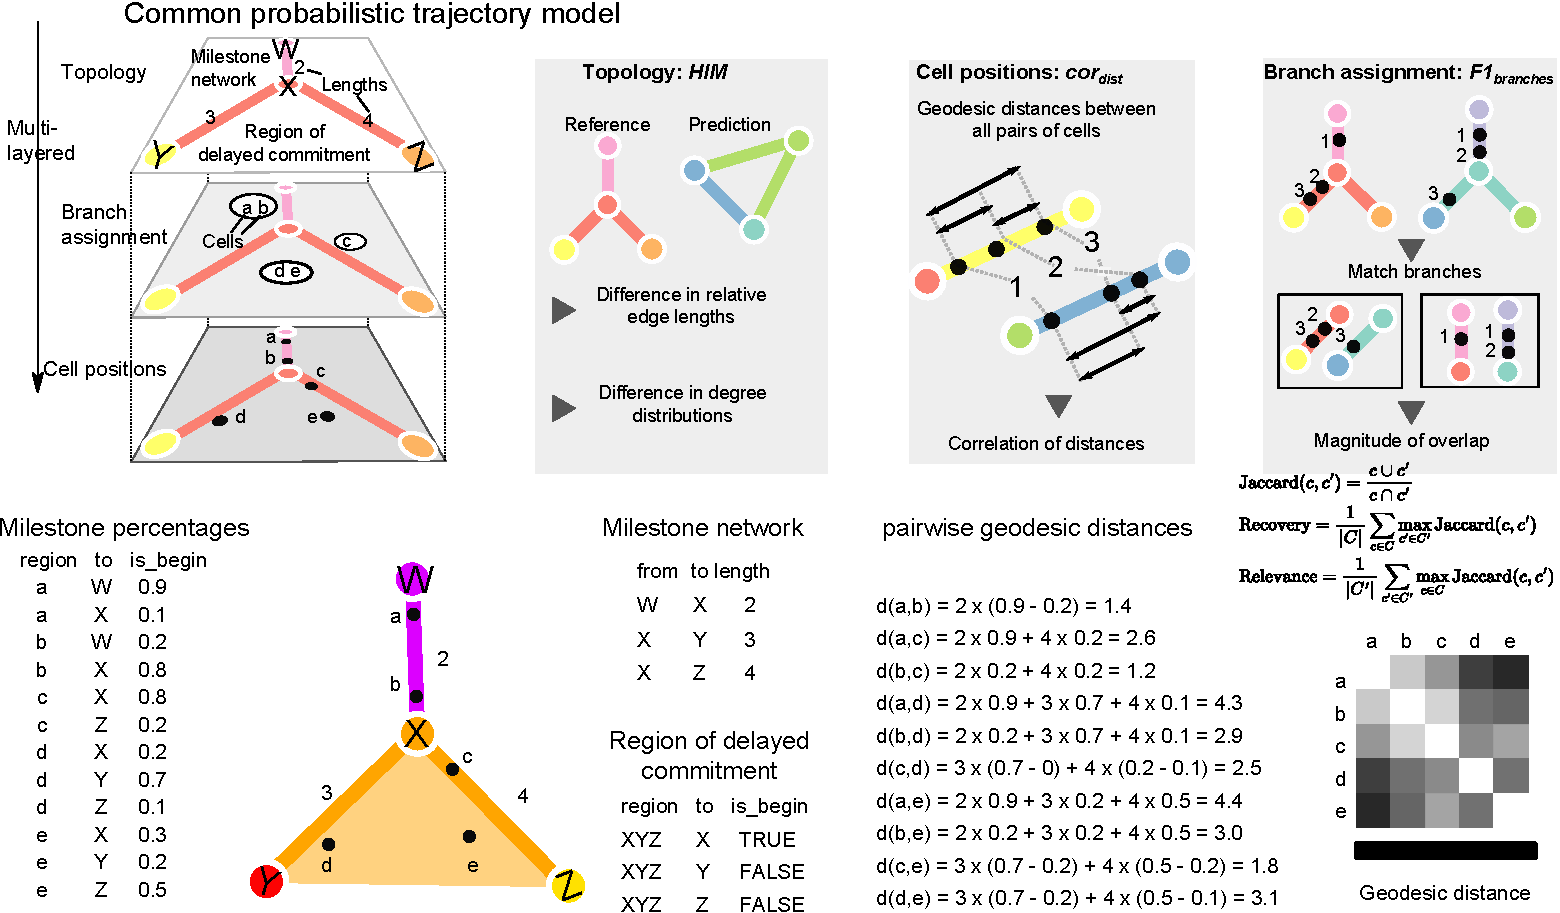
\includegraphics[width=0.95\textwidth]{dynverse_metrics/fig}
	\vspace{0.1cm}
	\caption[dynverse\_metrics]{
	dynverse\_metrics.}
	\label{fig:dynverse_metrics}
\end{figure}

\begin{figure}[!ht]
	\centering
	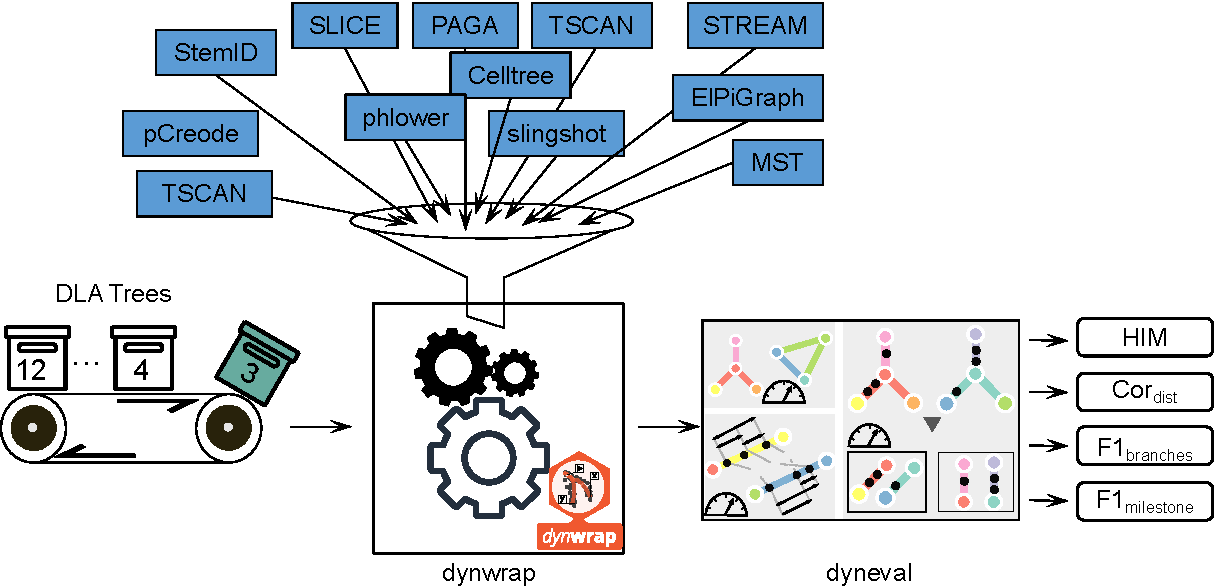
\includegraphics[width=0.95\textwidth]{evaluation_PHLOWER/fig}
	\vspace{0.1cm}
	\caption[evaluation\_PHLOWER]{
	evaluation\_PHLOWER.}
	\label{fig:evaluation_PHLOWER}
\end{figure}


\begin{figure}[!ht]
	\centering
	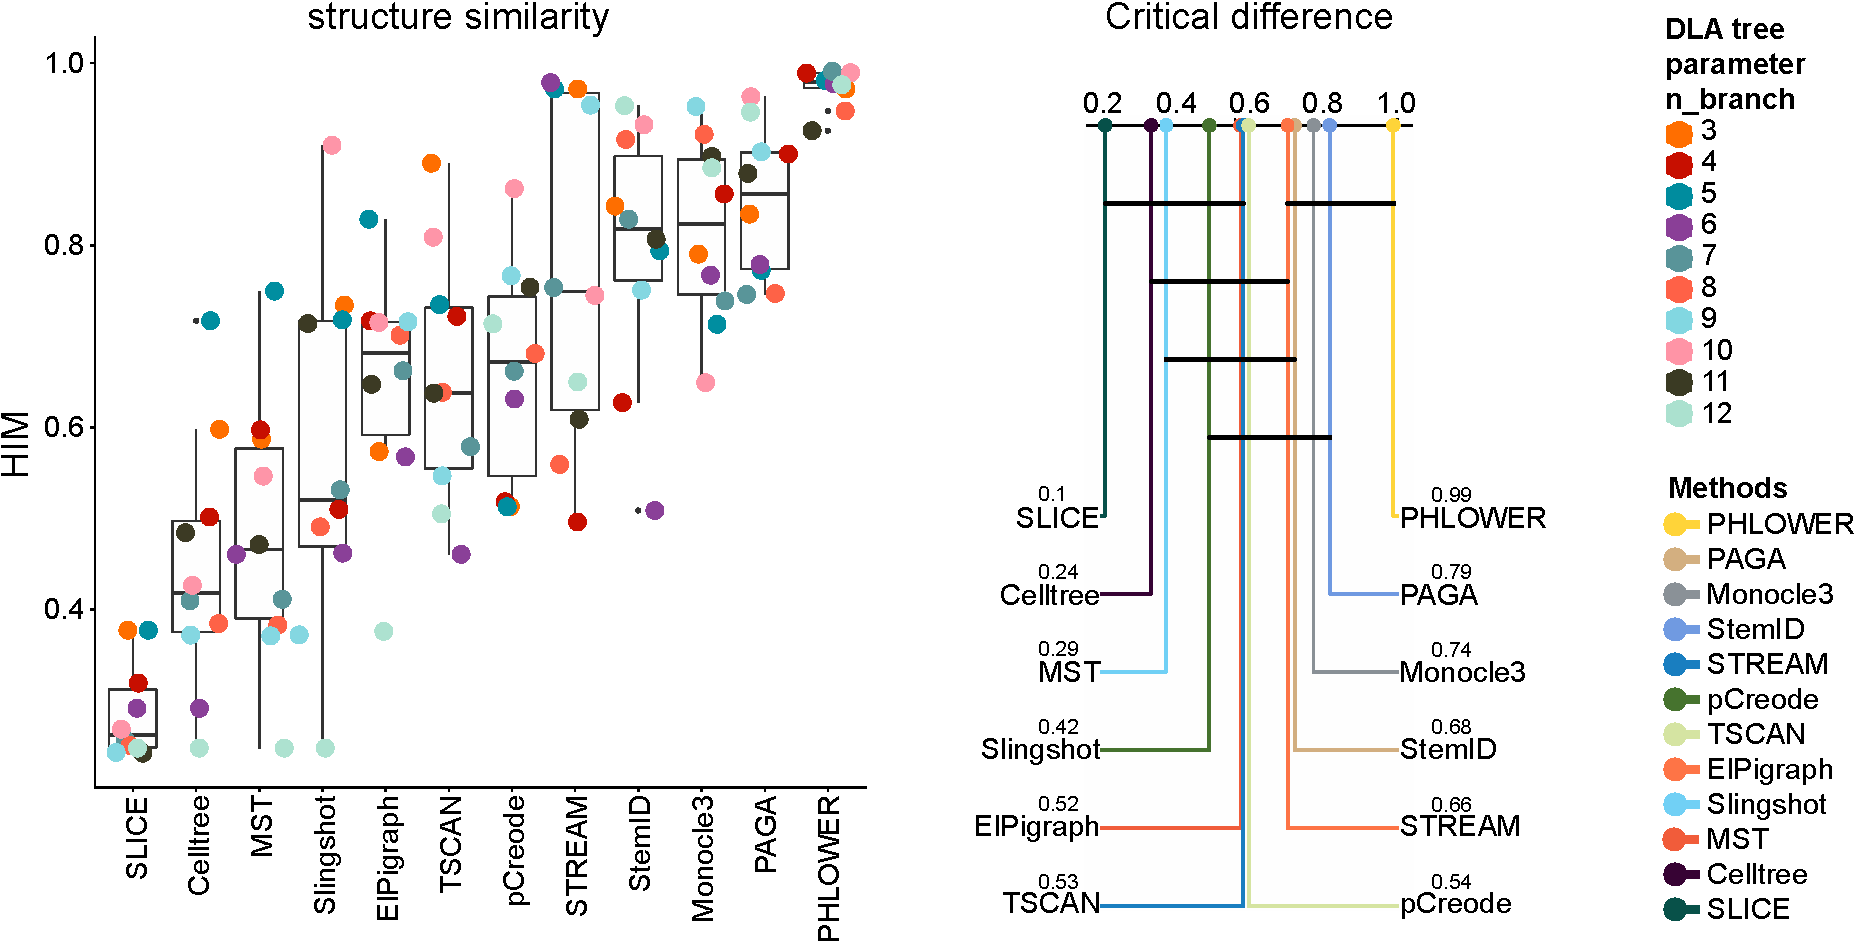
\includegraphics[width=0.95\textwidth]{HIM/fig}
	\vspace{0.1cm}
	\caption[Structure similarity benchmarking]{
	\textbf{Structure similarity benchmarking}.}
	\label{fig:HIM}
\end{figure}


\begin{figure}[!ht]
	\centering
	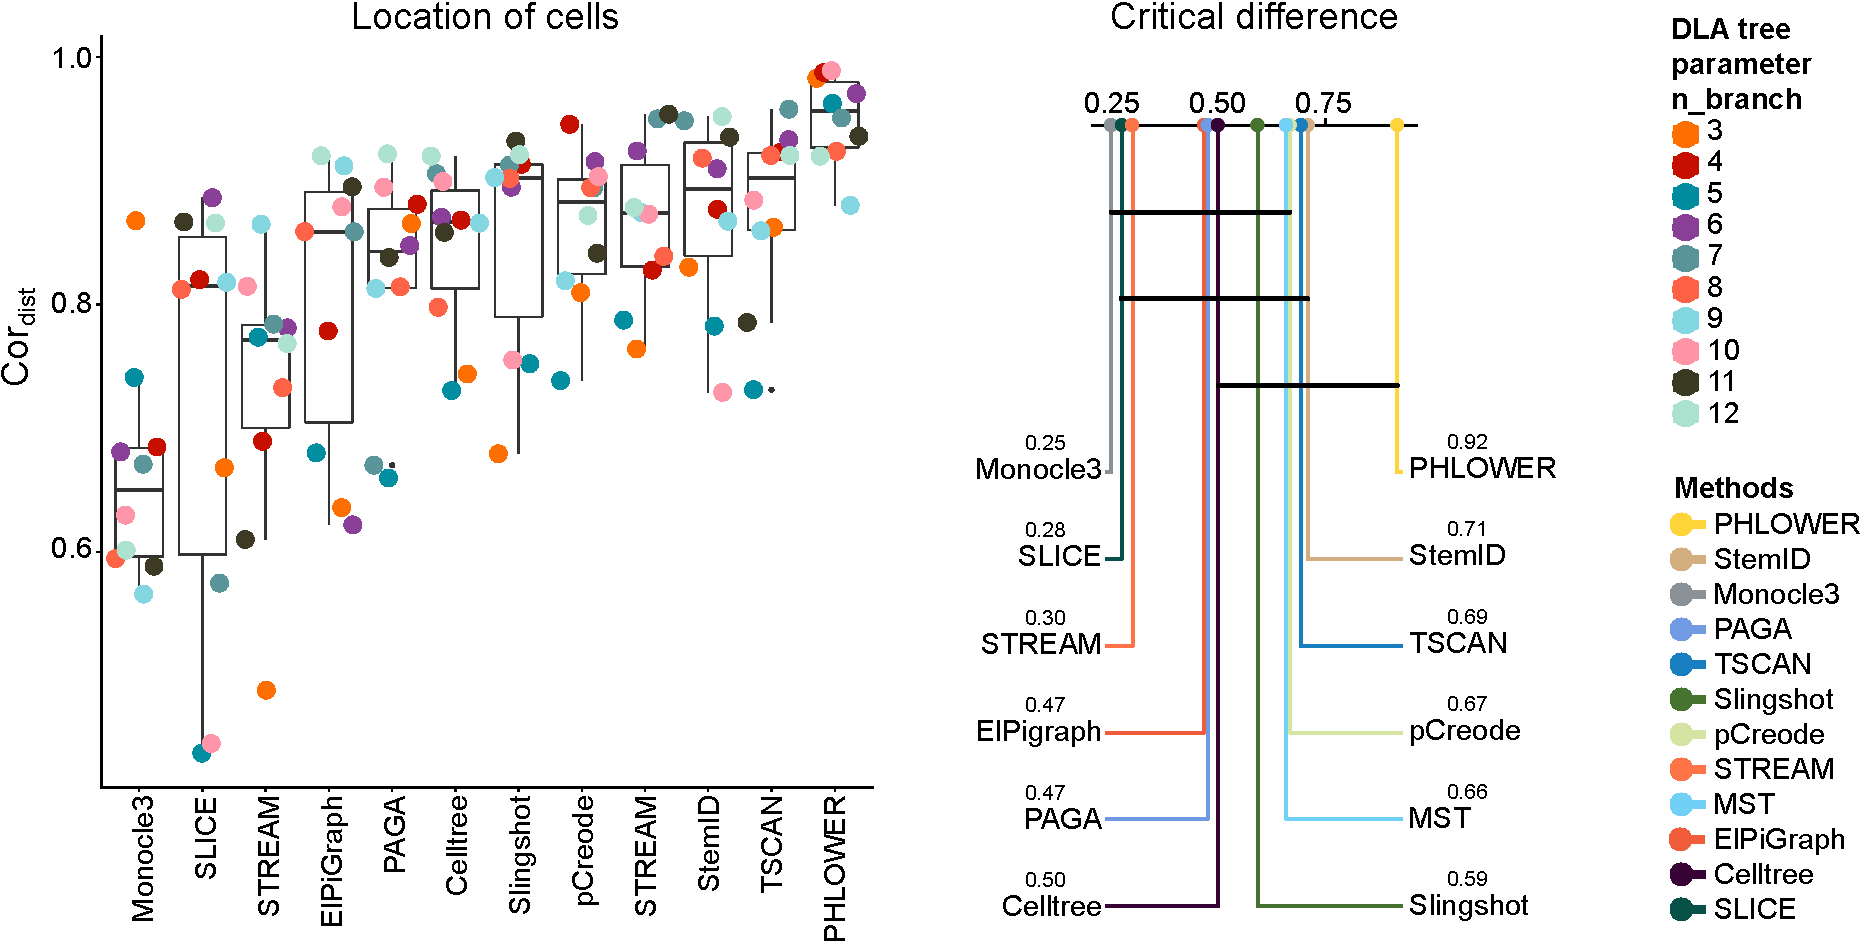
\includegraphics[width=0.95\textwidth]{Cordist/fig}
	\vspace{0.1cm}
	\caption[Location of cells]{
	\textbf{Location of cells}.}
	\label{fig:Cordist}
\end{figure}


\begin{figure}[!ht]
	\centering
	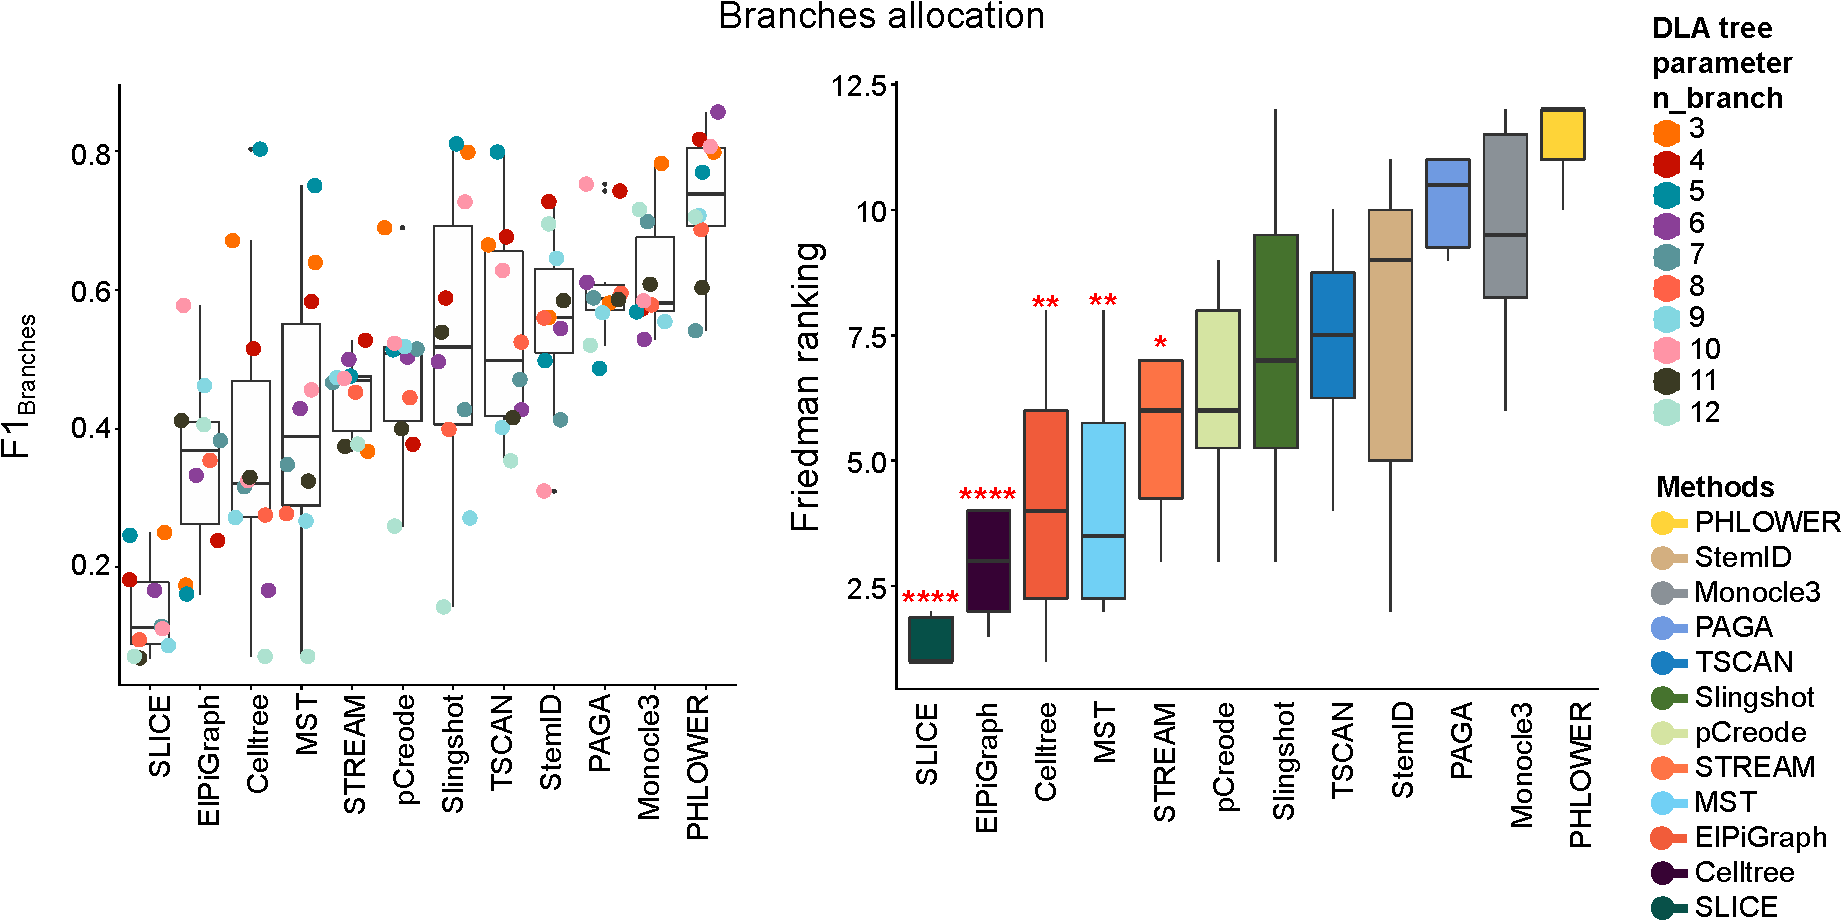
\includegraphics[width=0.95\textwidth]{F1branches/fig}
	\vspace{0.1cm}
	\caption[Branches allocation]{
	\textbf{Branches allocation}.}
	\label{fig:f1branches}
\end{figure}

\begin{figure}[!ht]
	\centering
	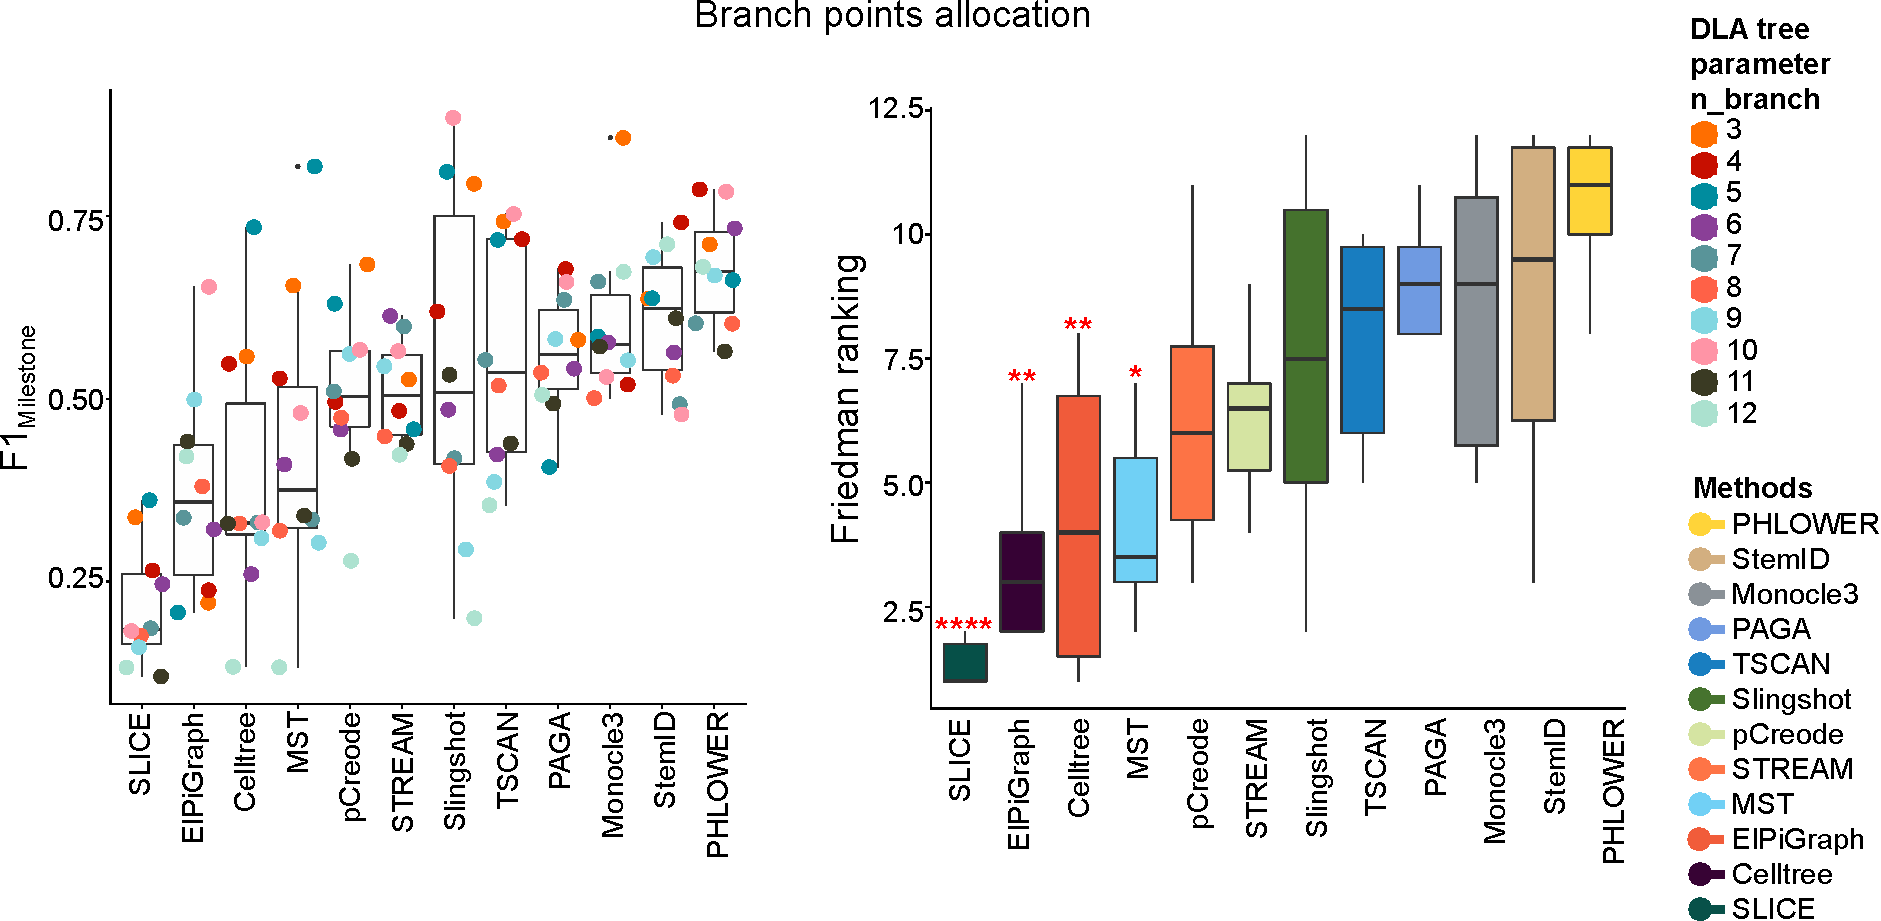
\includegraphics[width=0.95\textwidth]{F1milestone/fig}
	\vspace{0.1cm}
	\caption[Branch points allocation]{
	\textbf{Branch points allocation}.}
	\label{fig:f1milestone}
\end{figure}

\begin{figure}[!ht]
	\centering
	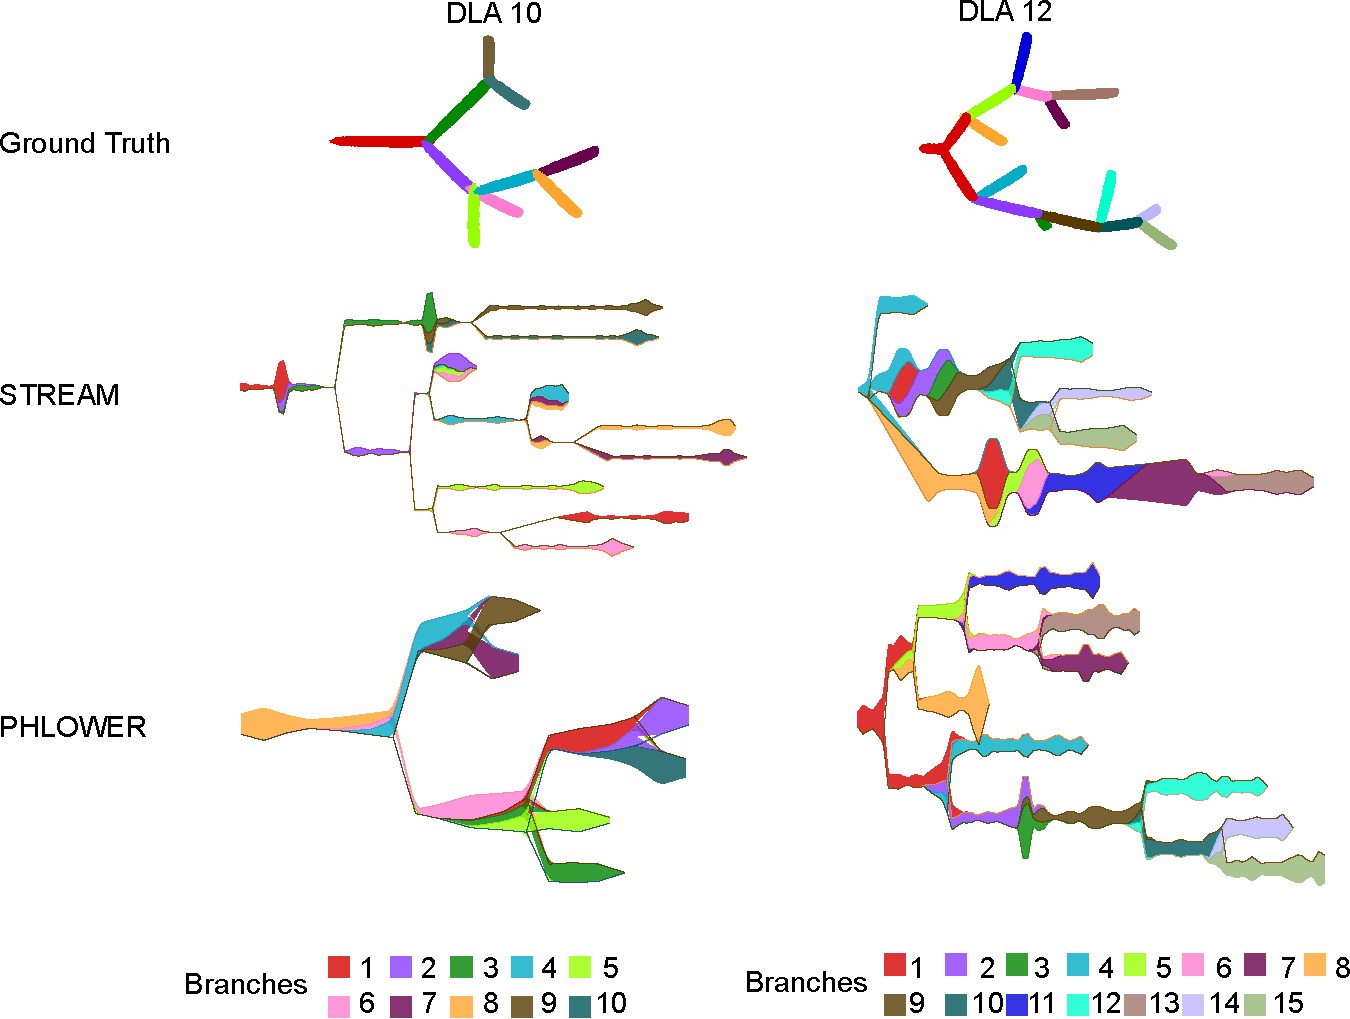
\includegraphics[width=0.95\textwidth]{PHLOWER_STREAM_layout/fig}
	\vspace{0.1cm}
	\caption[STREAM plots comparison]{
	\textbf{STREAM plots comparison}.}
	\label{fig:PHLOWER_STREAM}
\end{figure}



\section{Results}
\subsection{Apply Trajectory inference to kidney organoid data}
\subsection{Characterize the cell fate xxxx}

\section{Discussion}

